\documentclass[10pt]{beamer}
\usepackage{theme}
\usepackage[utf8]{inputenc}
\usepackage{subcaption}
\usepackage{tcolorbox}

\bibliographystyle{plain}
\newcommand{\venueyear}{QCNC, 2025}
\date{\venueyear}


\title{A Scalable Framework \\ for Post-Quantum Authentication  \\ in Public Key Infrastructures}
\author{%
Antonia Tsili\inst{1,2} \and 
Konstantinos Kordolaimis\inst{2} \and 
Konstantinos Krilakis\inst{2} \and
Dimitris Syvridis\inst{1,2}
}
% Renew command to be able to use linebreaks
\renewcommand{\insertshortauthor}{A. Tsili, K. Kordolaimis \\ K. Krilakis, D. Syvridis}
% Define short author version (for footer, navigation, etc.)
\institute[shortinst]{\inst{1} National and Kapodistrian University of Athens \and %
                      \inst{2} Eulambia Advanced Technologies}
\date{\venueyear}

\begin{document}
%------------------------------------------------
%------------------------------------------------
\begin{frame}[plain]
    \titlepage
    \vfill
    \titlepagefooter
\end{frame}
%------------------------------------------------
%------------------------------------------------
\begin{toc-title}
\begin{frame}[plain]{Contents}
    \tableofcontents
    \end{frame}
\end{toc-title}
%------------------------------------------------
%------------------------------------------------
\section{Introduction}
\begin{frame}{Quick background on PQC}
	The proven robustness of classical cryptography algorithms (e.g. RSA~\cite{RSA}), has resulted into their widespread adoption. Such algorithms' backbone adheres to similar mathematical guarantees, making them vulnerable to attacks from quantum computers. 
	
	\medskip 
	
	The National Institute of Standards and Technology (NIST) initiated in 2016 the concentration, trialling, assessment and standardization of post-quantum cryptography (PQC) algorithms in view of these security attacks. 
	
	\medskip 

	Research is focused on four NIST standardization finalists, including CRYSTALS-Kyber for key establishment~\cite{Kyber}, \textbf{CRYSTALS-Dilithium} \cite{Dilithium}, \textbf{Falcon}~\cite{prest2020falcon} and \textbf{SPHINCS$^+$}~\cite{Sphincs} for digital signatures. 
\end{frame}
%------------------------------------------------
%------------------------------------------------
\begin{frame}[allowframebreaks]{Description of PKI}
\vfill
\textcolor{blue!30!red!90}{We create a framework that can assist in transitioning current PKI topologies to the post-quantum era.}
\medskip
\begin{tcolorbox}[
	colframe = blue!30,
	colback  = blue!8
	]%%
	PKI refers to a system that functions through the management and usage of certificates.
	\begin{itemize}
		\item Network entities bear signed certificates.
		\item The certificates are signed by well-known and trusted Certificate Authorities (CA).
		\item The signature is produced using the CA private key and can be verified using the CA public key.
	\end{itemize}
\end{tcolorbox}
\vfill

\break 

At top level of the chain-of-trust lies the \textbf{root CA} and at the bottom level are the \textbf{End Entities (EEs)}. There can be zero or more levels in-between connecting them, which comprise the \textbf{intermediate CAs (iCAS)}. The iCAs receive certificates from the parent levels' CAs specifying that they can themselves produce certificates for the child levels' iCA's/EEs.

\medskip

\begin{columns}[T]	
	\column{0.45\textwidth}
	\medskip
	
	The certificates are used for \textbf{authenticating} peers before information exchange. An entity that owns a certificate bearing a CA's verified signature is considered secure, therefore, identity can be proved through the signed certificate.
	
	\column{0.5\textwidth}
	\begin{figure}
		\begin{center}
		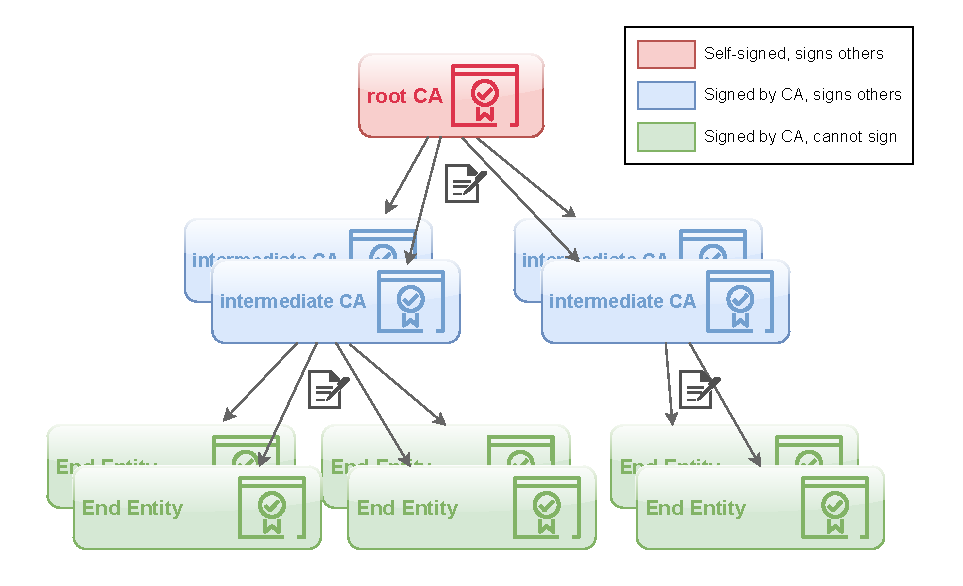
\includegraphics[width=\textwidth]{images/PKI.drawio.pdf}
		\end{center}
	\end{figure}
	\smallskip
\end{columns}
\end{frame}


\section{Contributions}
%------------------------------------------------
%------------------------------------------------
\begin{frame}{Contributions}
	\begin{itemize}
		\item \textbf{Scalable certificate authority employing PQC signatures} to manage a large client base requesting certificates signed with PQC signature algorithms.
		\item \textbf{Classical and PQC compatibility and adaptability} by accommodating both new and classical algorithms on-the-fly.
		\item \textbf{Automated certificate issuance with PQC signatures} to automate issuance and verification of digital certificates using PQC signature algorithms.
		\item \textbf{Hierarchical three-layer architecture on a full-fledged network simulation including 3 layers -- CA, iCA, and EEs} to promote certificate management and scalability (e.g. for QKD topology).
		\item \textbf{Performance metrics for operations including certificates} to compare performance metrics on signing, verifying, and distributing certificates across multiple clients.
		\item  \textbf{Crypto-agility promotion} by lifting PQC requirements at the client level.
	\end{itemize}
\end{frame}


\section{Methodology}
%------------------------------------------------
%------------------------------------------------
\begin{frame}{Overview of the framework}
	We create a scalable and extensible prototype framework comprising a CA and an automatic certificate issuance system, where all CA components included can easily switch from classical to PQC signatures and back. 
	
	\medskip
	
	We distinguish the framework's function between the levels of the root CA, the iCAs and the EEs, with services distributed to serve each level accordingly. 
	The root CA activity is distributed into three services aimed at serving the iCAs' requests. 
	
	\medskip
		
	\textbf{Our design isolates different chains-of-trust forming across the levels -- if one iCA/EE is comprimised, peers of the same and upper levels will not be affected.}
	
\end{frame}
%------------------------------------------------
%------------------------------------------------
\begin{frame}[allowframebreaks]{Root CA}

	\medskip

	\begin{columns}[T]	
		\column{0.45\textwidth}
		
		We assume that potential iCAs are pre-registered in a database for security purposes -- unknown iCAs cannot be served. The iCA \textsc{POST}s its information at the \textit{enroll} endpoint of the enrollment service. The service generates a new certificate dedicated to the iCA client, preserving the integrity of each certificate chain.
		\hfill\break 
		
		The iCA produces a certificate signing request (CSR), logs in the \textit{certify} service, receives a timed token and \textsc{POST}s the CSR and token. 
		
		\column{0.5\textwidth}
		The root CA responds with the iCA's signed certificate, which expects it sent back for monitoring. The iCA can use the \textit{verify} service to validate the certificate chain, when an EE requests the issuance of a certificate.
		
		\medskip 
		
		\begin{figure}
		\centering
		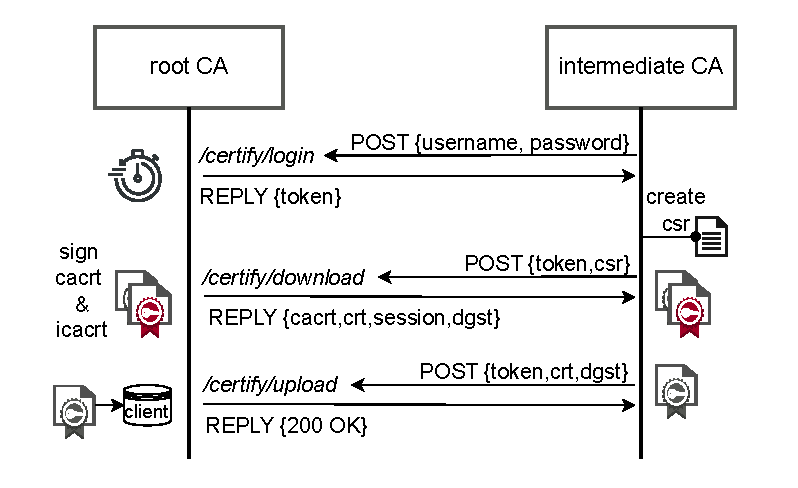
\includegraphics[width=\textwidth]{images/CAendpoints.drawio.pdf}
		\end{figure}
		\smallskip
	\end{columns}

\end{frame}
%------------------------------------------------
%------------------------------------------------
\begin{frame}[allowframebreaks]{Intermediate CA}
	
	The iCAs' service design is similar to the root CA's.
	
	\begin{columns}[T]	
		\column{0.45\textwidth}
		The EE enrolls to the iCA. The iCA creates and sends its CSR to the root CA. The new iCA certificate will be a part of the particular chain-of-trust.
		\hfill\break 
		
		The client produces a CSR and logs in the iCA's certify service. The iCA verifies its own certificate and signs the EE's certificate. The iCA sends the EE's certificate and expects to receive it back as confirmation.
		
		\column{0.5\textwidth}
		The iCA can use the \textit{verify} service to validate the certificate chain, when an EE requests the issuance of a certificate.
		
		\medskip 
		
		\begin{figure}
			\centering
			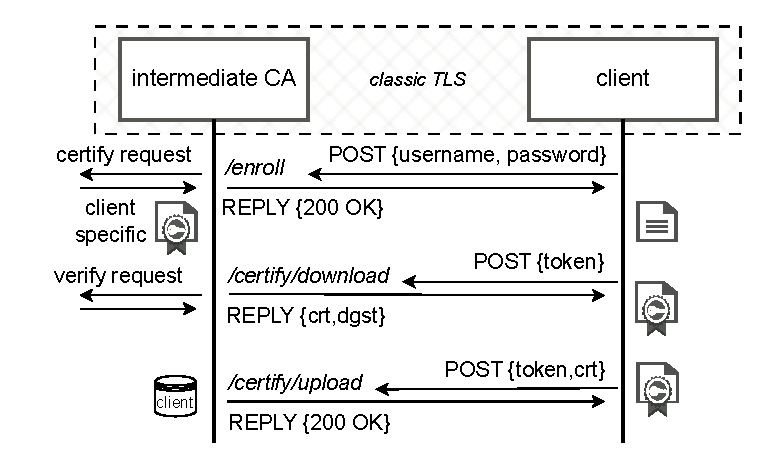
\includegraphics[width=\textwidth]{images/iCAclient.drawio.pdf}
		\end{figure}
		\smallskip
	\end{columns}
\end{frame}

\section{Experiments}
%------------------------------------------------
%------------------------------------------------
\begin{frame}{Description of Experiments}
	We test our system by performing two sets of experiments on the employment of PQC signature algorithms for certificate issuance. In both cases, we use Dilithium, SPHINCS$^+$ and Falcon variants to produce certificates on the topologies described in the following.  
	
	\begin{itemize}
		\item[$\blacktriangleright$] The root CA is PQC-enabled, while the root CA and two different iCAs located at separate terminals. Each iCA receives requests from 25,50,100,250 and 500 natively located clients concurrently, and then produces the matching requests addressed to the root CA according to the workflow described before.
		\item[$\blacktriangleright$] Both root CA and iCAs are PQC-enabled. The iCA is placed at Machine 1 and clients at Machine 2 and Machine 3. The iCA receives requests from 50,100,200,500 and 1000 remotely located clients concurrently, and then produces the matching requests addressed to the root CA. 
	\end{itemize}

\end{frame}	
%------------------------------------------------
%------------------------------------------------
\begin{frame}{Measurements}
	We measure the time taken to complete the following operations as the number of clients increase.
	
	\begin{columns}[T]	
		\column{0.45\textwidth}
		\begin{itemize}
			\item iCA certificate issuance, including:
			\begin{enumerate}
				\item iCA download (send CSR, root CA sign, receive certificate)
				\item iCA upload (send certificate to root CA)
			\end{enumerate}
			\item client certificate issuance, including:
			\begin{enumerate}
				\item iCA certificate verification
				\item client (send client's CSR, iCA sign, receive certificate)
				\item client upload (send certificate to iCA)
			\end{enumerate}
		\end{itemize}
		\column{0.45\textwidth}
		\begin{itemize}
			\item root CA signign iCA certificate.
			\item root CA verifying iCA's certificate.
		\end{itemize}
		\begin{figure}
			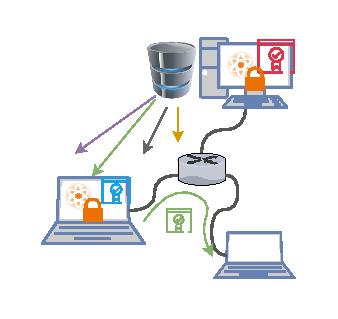
\includegraphics[width=.8\textwidth,trim={0.5cm 0.5cm 0.5cm 0.5cm},clip]{images/topology.drawio.pdf}
		\end{figure}
	\end{columns}
	
\end{frame}
%------------------------------------------------
%------------------------------------------------
\begin{frame}[allowframebreaks]{Results}
	
	\begin{itemize}
		\item SPHINCS$^+$' verification time remains relatively low
		\item ``heavier'' Falcon variant is quicker than the ``lighter'' variant producing for the overall client certificate production
		\item caching accelerates overall process for ``heavier'' algorithms
	\end{itemize}
	
	\begin{columns}[T]	
		\column{0.5\textwidth}
		\begin{figure}
			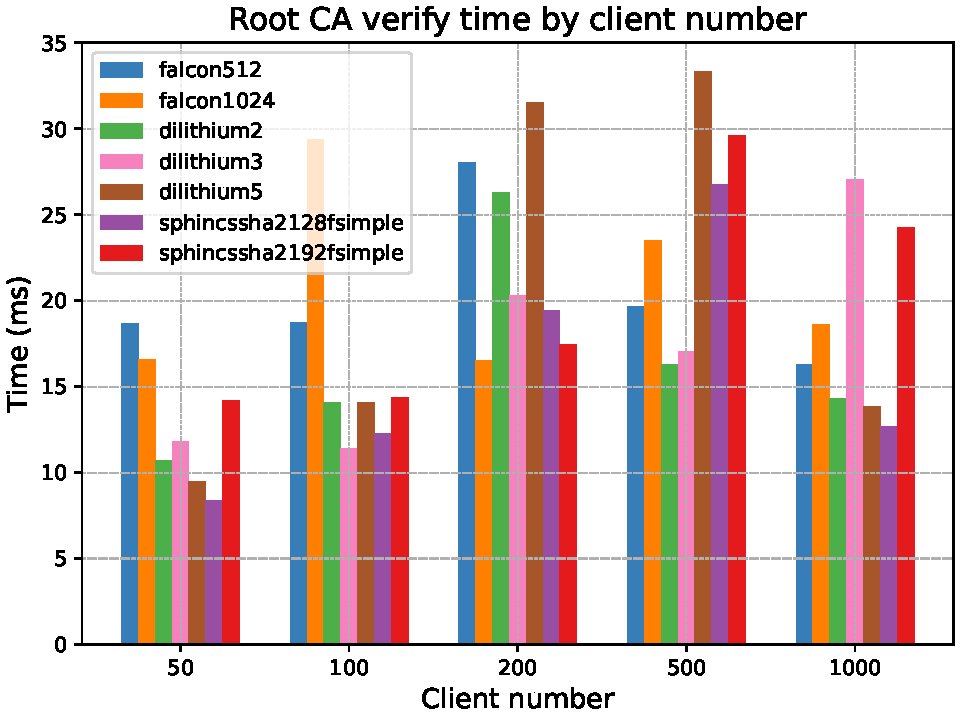
\includegraphics[width=\textwidth]{images/verify_means.pdf}
		\end{figure}
		\column{0.5\textwidth}
		\begin{figure}
			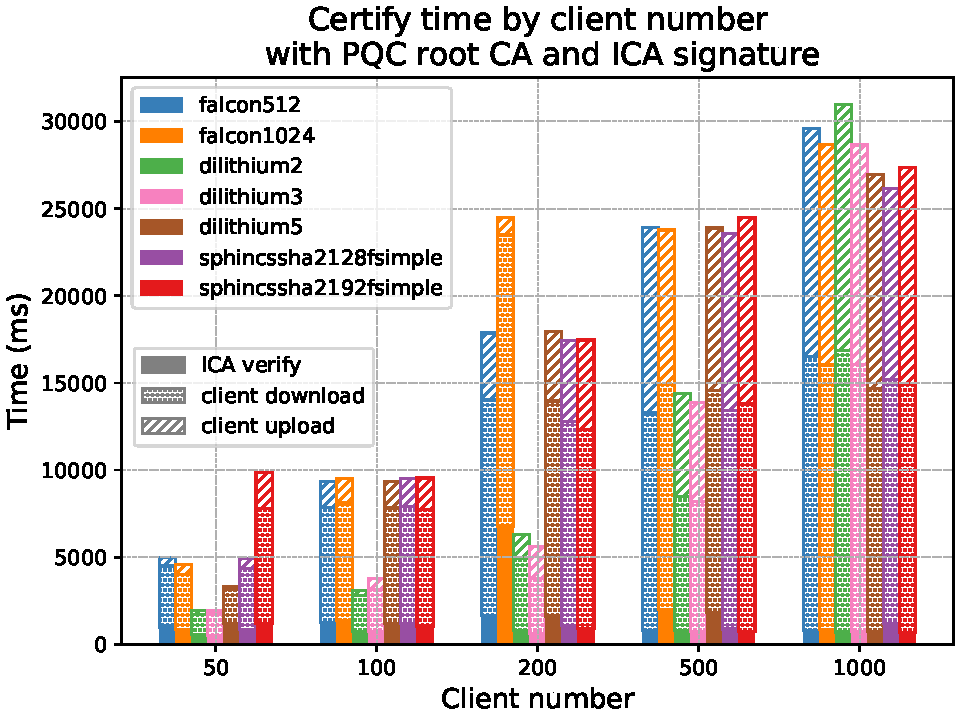
\includegraphics[width=\textwidth]{images/client_means_2PQC.pdf}
		\end{figure}
	\end{columns}
	
	\break

	\begin{itemize}
		\item The workflow we design places computational burden on verifying certificates at levels usually comprising heavy-duty computers, making the SPHINCS$^+$ variants a sensible choice.
		\item Caching helps accelerate processes for algorithms with large keys.
		\item The Dilithium variants encounter significant overhead  as the number of clients grows.
	\end{itemize}
\end{frame}
%------------------------------------------------
%------------------------------------------------
\begin{frame}[allowframebreaks]{Extensions and future work}
	
	\emph{We are currently working on scaling and securing our framework, while forming a robust architecture with extensive monitoring properties.}
	
	\medskip
	
	\begin{enumerate}
		\item \textbf{Root CA breaks into multiple CAs; each CA signs a certificate per functionality.}
		
		As the framework scales to serve different clients from different domains, more sophisticated horizontal organization is essential. Multiple certificates are signed according to the recipient's role, functionality and permissions.
		\hfill\break
		
		\item \textbf{Control of EEs is handed over to domains}
		
		Each domain comprises EEs/clients that correspond to different chains-of-trust. EEs are organized into groups depending on the domain they belong. Certificate distribution and status is, then, administrated per domain.
		
		\break
		\item \textbf{Services are decoupled from network components}
		
		Services are treated as a separate entity inside the network, existing beyond physical network components. This allows their dynamic configuration and easy maintenance.
		\hfill\break
		
		\item \textbf{Maintenance is automated and monitoring is better facilitated}
		Monitoring is carried out using state-of-the-art tools utilizing time series records, which allows for triggering automated maintenance procedures. All domains produce data that can help monitor the entire framework, as well as illustrate its functionality. 
		\hfill\break
		
		\item \textbf{The system architecture will follow a software-defined network management (SDN).}
	\end{enumerate}
\end{frame}
%------------------------------------------------
%------------------------------------------------
\begin{frame}[allowframebreaks]{References}
	\bibliography{references}
\end{frame}

\end{document}